\graphicspath{{introduction/fig/}}

\chapter{Introduction}
\label{chap:introduction}

The last few years have seen great advances in speech recognition. Much of this progress is due to the resurgence of neural networks; most speech systems now rely on deep neural networks (DNNs) with millions of parameters~\cite{dahl+etal_taslp12,hinton+etal_spm2012}.
However, as the complexity of these models has grown, so has their reliance on labelled training data. Currently, system development requires large corpora of transcribed speech audio data, texts for language modelling, and pronunciation dictionaries.
Despite speech applications becoming available in more languages, it is hard to imagine that resource collection at the required scale would be possible for all 7000 languages spoken in the world today.

I really like apples.

\section{Section heading}

This is some section with two table in it: Table~\ref{tbl:exemplars} and Table~\ref{tbl:abx_speaker}.

\begin{table}[!h]
    \mytable
    \caption{Performance of the unconstrained segmental Bayesian model on TIDigits1 over iterations in which the reference set is refined.}
    \begin{tabularx}{\linewidth}{@{}lCCCCC@{}}
        \toprule
        Metric     & 1 & 2 & 3 & 4 & 5 \\
        \midrule
        WER (\%)                        & $35.4$ & $23.5$ & $21.5$ & $21.2$ & $22.9$ \\
        Average cluster purity (\%)       & $86.5$ & $89.7$ & $89.2$ & $88.5$ & $86.6$ \\
        Word boundary $F$-score (\%)         & $70.6$ & $72.2$ & $71.8$ & $70.9$ & $69.4$ \\
        Clusters covering 90\% of data   & 20             & 13 & 13 & 13 & 13 \\
        \bottomrule
    \end{tabularx}
    \label{tbl:exemplars}
\end{table}


\begin{table}[!h]
    \renewcommand{\arraystretch}{1.1}
    \centering
    \caption{A table with an example of using multiple columns.}
    \begin{tabularx}{0.65\linewidth}{@{}lCCr@{}}
        \toprule
        & \multicolumn{2}{c}{Accuracy (\%)} \\
        \cmidrule(lr){2-3}
        Model    & Intermediate & Output & Bitrate\\
        \midrule
        Baseline & 27.5         & 26.4   & 116 \\
        VQ-VAE   & 26.0         & 22.1   & 190 \\
        CatVAE   & 28.7         & 24.3   & 215 \\
        \bottomrule
    \end{tabularx}
    \label{tbl:abx_speaker}
\end{table}

\newpage

This is a new page, showing what the page headings looks like, and showing how to refer to a figure like Figure~\ref{fig:cae_siamese}.

\begin{figure}[!t]
    \centering
%     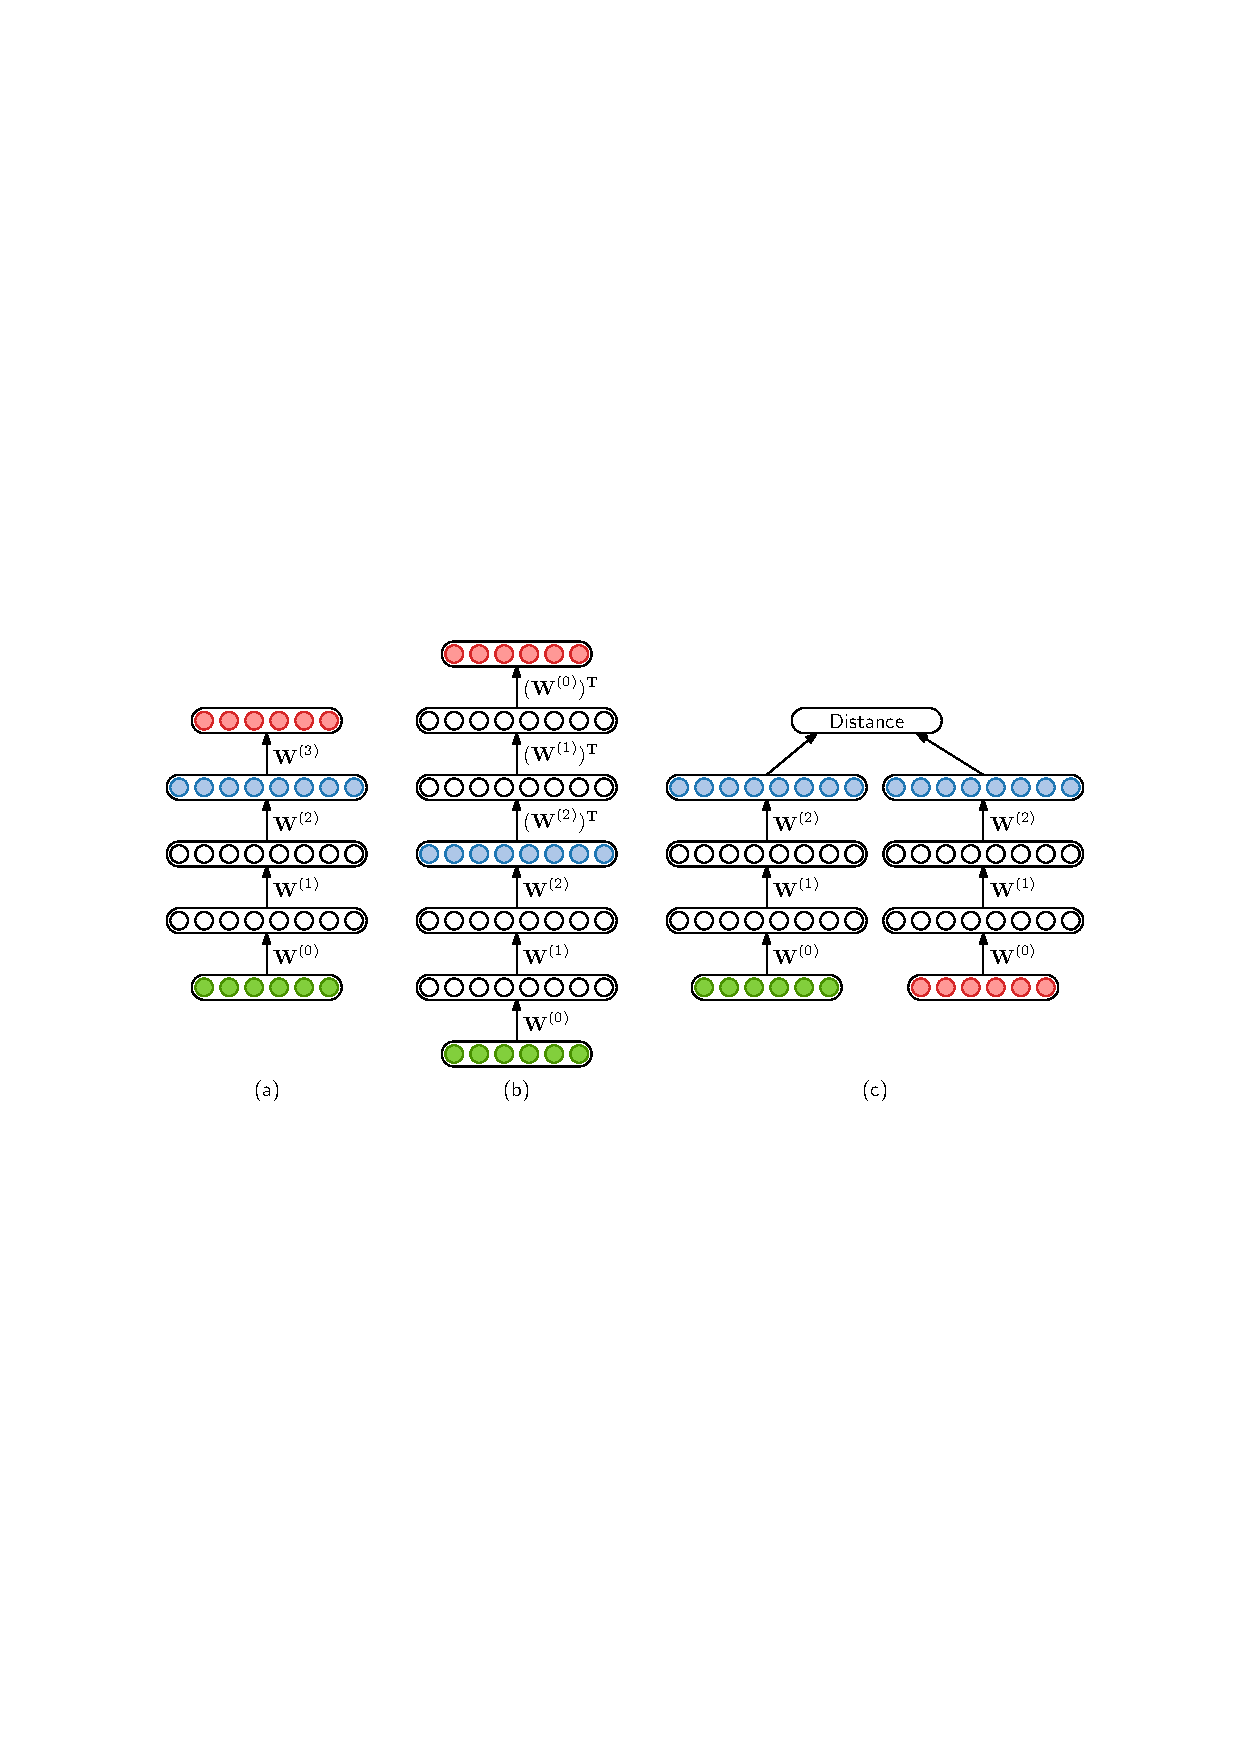
\includegraphics[width=\linewidth]{cae_siamese}
    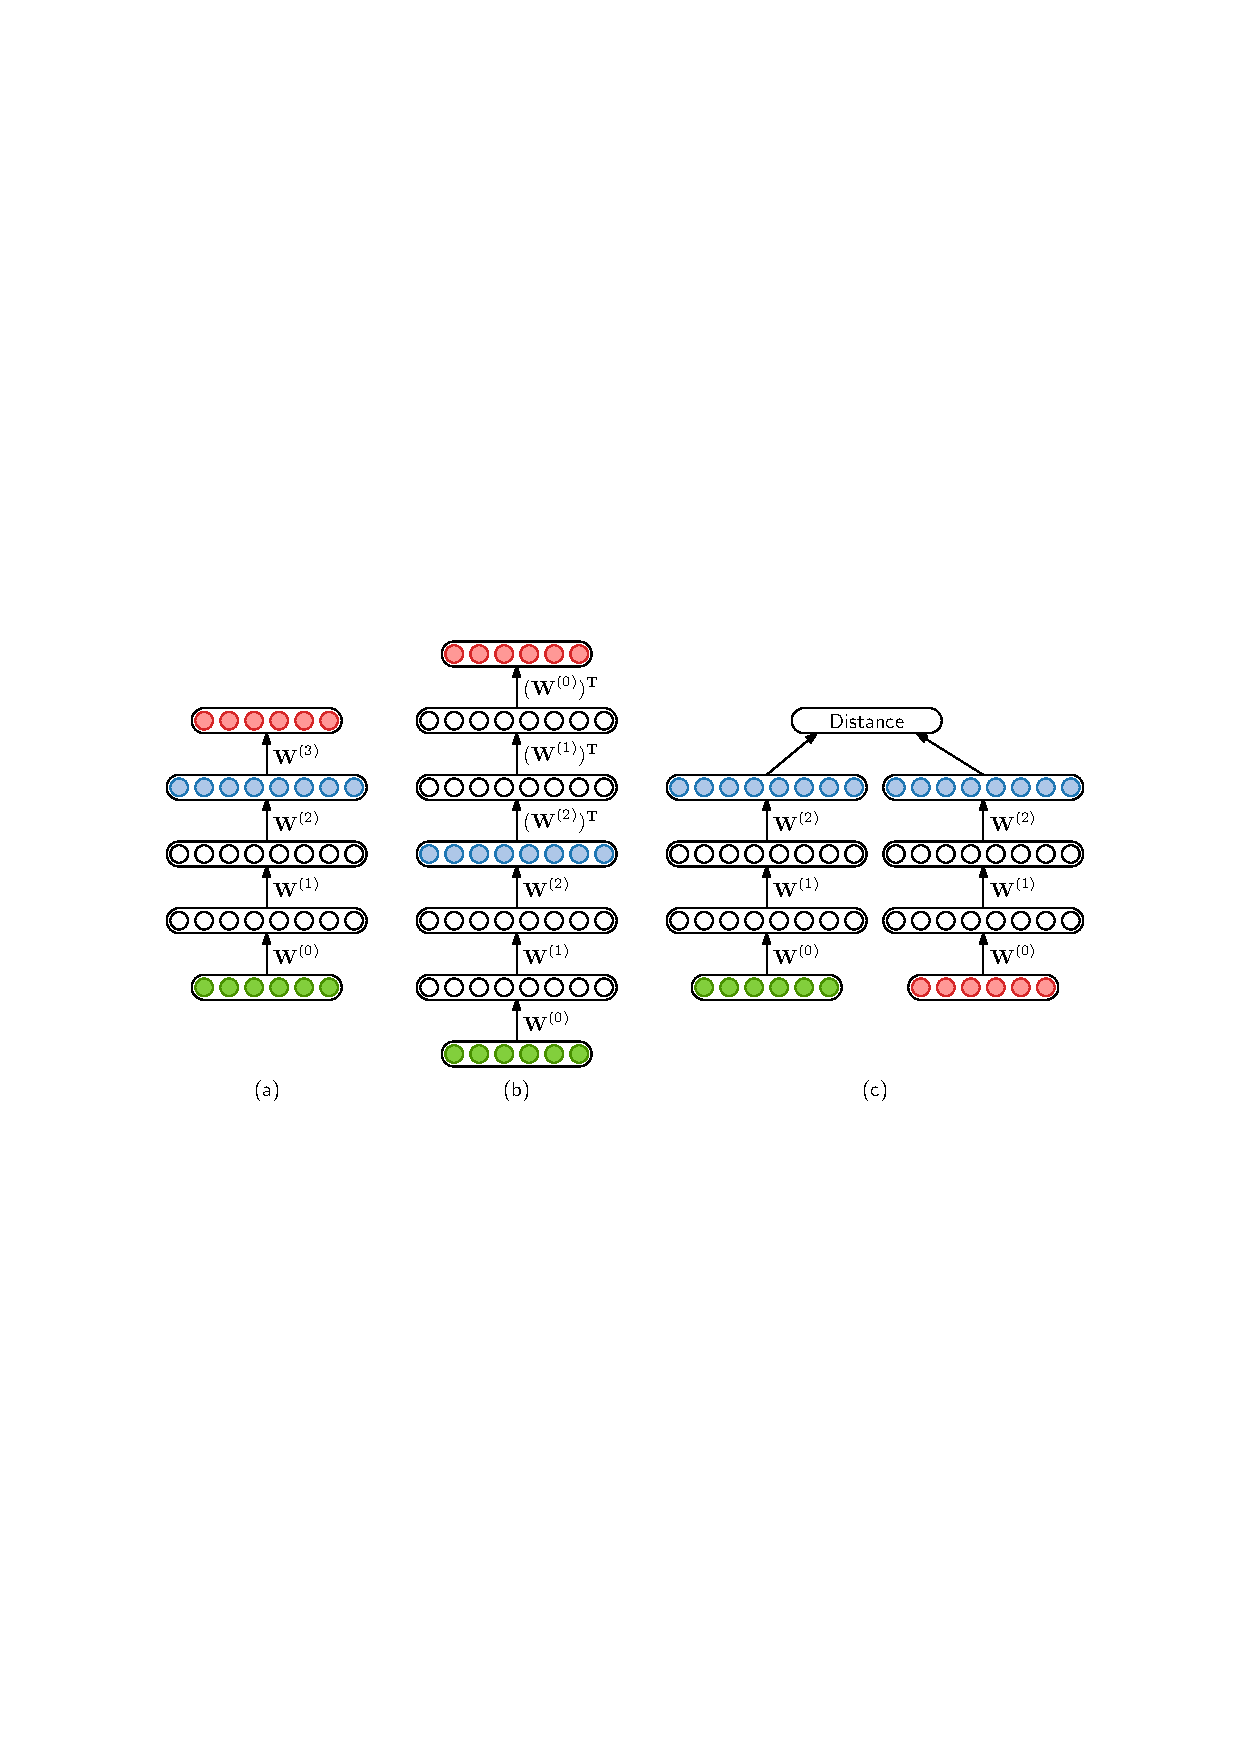
\includegraphics[width=0.918\linewidth]{cae_siamese}
    \caption[I am the short caption that appears in the list of figures, without references.]{
    (a) The cAE as used in this chapter. The encoding layer (blue) is chosen based on performance on a development set.
    (b) The cAE with symmetrical tied weights. The encoding from the middle layer (blue) is always used.
    (c) The siamese DNN. The cosine distance between aligned frames (green and red) is either minimized or maximized depending on whether the frames belong to the same (discovered) word or not.
    A cAE can be seen as a type of DNN~\cite{dahl+etal_taslp12}.
    }
    \label{fig:cae_siamese}
\end{figure}


The following is an example of an equation:
\begin{equation}
P(\vec{z} | \vec{\alpha}) = \int_{\vec{\pi}} P(\vec{z} | \vec{\pi}) \, p(\vec{\pi} | \vec{\alpha}) \, \textrm{d} \vec{\pi}
= \int_{\vec{\pi}} \prod_{k = 1}^K \pi_k^{N_k} \frac{1}{B(\vec{\alpha})} \prod_{k = 1}^K \pi_k^{\alpha_k - 1} \, \textrm{d} \vec{\pi}
\label{eq:example_equation}
\end{equation}
which you can subsequently refer to as~\eqref{eq:example_equation} or Equation~\ref{eq:example_equation}.
But make sure to consistently use the one or the other (and not mix the two ways of referring to equations).
